% 2023年北京高考数学第15题解析图3：a=4/5时的距离极值分析
\begin{tikzpicture}[>=stealth,line width=0.6pt,font=\normalsize]
  \draw[->] (-2.2,0) -- (2.2,0) node[below] {$x$};
  \draw[->] (0,-1.8) -- (0,1.8) node[left] {$y$};
  \node[below left] at (0,0) {$O$};

  % 半圆
  \draw (1.0,0) arc[start angle=0,end angle=180,radius=1.0];
  \node[below] at (-1.0,0) {$-\dfrac{4}{5}$};
  \node[below right] at (1.0,0) {$\dfrac{4}{5}$};

  % 左侧分支
  \draw[dashed] (-1.0,0) -- (-1.0,1.4);
  \draw (-2.0,0.4) -- (-1.0,1.4);
  \draw[fill=white] (-1.0,1.4) circle (1.5pt);

  % 右侧分支
  \draw[dashed] (1.0,0) -- (1.0,-1.3);
  \draw (1.0,-1.3) -- (1.9,-1.8);
  \draw[fill=white] (1.0,-1.3) circle (1.5pt);

  % 垂线段 OP 与交点 Q
  \coordinate (P) at (-1.2,1.2);
  \coordinate (Q) at (-0.707,0.707);
  \draw (0,0) -- (P);
  \node[above left] at (P) {$P$};
  \node[above right] at (Q) {$Q$};
\end{tikzpicture}
